% p22-h-completes-the-following-diagram.tex
%
% Source:   Carl A. Gunter and Dana S. Scott, "Semantic Domains".
%           ScottDomains/papers/Gunter Scott 1990.pdf
% Physical page: 22          Printed page: 21
% Section:  4.4 Sums and lifts. (immediately before 4.5)
% Unnamed in the paper (no figure number). Introduced by:
%   "Given cpo's D and E, we define the separated sum D + E to be the cpo
%    D_bot (+) E_bot. By the universal properties for (+) and (.)_bot, we know
%    that h = [f-dagger, g-dagger] is the unique strict continuous function
%    which completes the following diagram:"
%
% Content: the same shape as the coalesced-sum diagram on page 20, with the
% coprojections relabelled inl o up and inr o up and the sum written D + E.
% Vertices 4, arrows 5 (4 solid, 1 dashed). The paper adds immediately after:
% "However, h may not be the only continuous function which completes the
% diagram."
%
% Geometry measured from a 300 dpi render of the region and divided by
% 118.11 px/cm.
%
\documentclass[border=6pt]{standalone}
\usepackage{tikz}
\begin{document}
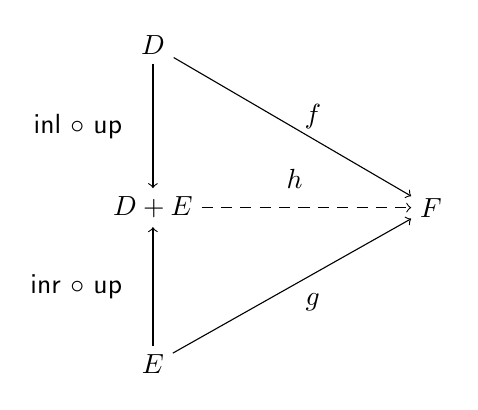
\begin{tikzpicture}[
  x=1cm, y=1cm,
  every node/.style={inner sep=1pt},
  open/.style={circle, draw, fill=white, minimum size=4pt, inner sep=0pt},
  solid/.style={circle, draw, fill=black, minimum size=5pt, inner sep=0pt},
  edge/.style={draw, line width=0.4pt},
  % added for the commutative diagrams: object nodes, and the paper's two
  % arrow kinds -- solid for a named map, dashed for the unique completing map
  obj/.style={inner sep=3pt},
  arrow/.style={draw, line width=0.4pt, ->},
  darrow/.style={draw, line width=0.4pt, ->, dash pattern=on 4pt off 3pt}]

  % vertices
  \node[obj] (d)   at (0.00, 2.06) {$D$};
  \node[obj] (sum) at (0.00, 0.00) {$D + E$};
  \node[obj] (e)   at (0.00,-1.99) {$E$};
  \node[obj] (f)   at (3.53, 0.00) {$F$};

  % arrows
  \draw[arrow]  (d)   -- (sum);
  \draw[arrow]  (e)   -- (sum);
  \draw[arrow]  (d)   -- (f);
  \draw[arrow]  (e)   -- (f);
  \draw[darrow] (sum) -- (f);

  % labels printed inside the picture
  \node[anchor=east]  at (-0.35, 1.03) {\textsf{inl} $\circ$ \textsf{up}};
  \node[anchor=east]  at (-0.35,-1.00) {\textsf{inr} $\circ$ \textsf{up}};
  \node                at (2.03, 1.16) {$f$};
  \node                at (2.03,-1.20) {$g$};
  \node[anchor=south] at (1.80, 0.20) {$h$};
\end{tikzpicture}
\end{document}
